\sloppy
\documentclass[14pt,a4paper,oneside]{extarticle}	% Размер основного шрифта и формата листа
\usepackage{xltxtra}						% Используется для вывода логотипа XeLaTeX
\usepackage{xunicode}						% Кодировка документа
\usepackage{polyglossia}					% Загружает пакет многоязыковой верстки
\newfontfamily\russianfont{Book Antiqua}
%\setmainfont{Liberation Serif}						% Основной шрифт текста
\setmainfont{Book Antiqua}
\setdefaultlanguage{russian}				% Основной язык текста
\setotherlanguage{english}					% Дополнительный язык текста
\linespread{1}							% Межстрочный интервал выбран полуторным
\usepackage[left=2.5cm,
right=1.5cm,vmargin=2.5cm]{geometry} % Отступы по краям листа
\bibliographystyle{ugost2008}

\usepackage{xcolor}
\usepackage{hyperref}
% Цвета для гиперссылок
\definecolor{linkcolor}{HTML}{359B08} % цвет ссылок
\definecolor{urlcolor}{HTML}{799B03} % цвет гиперссылок
\hypersetup{pdfstartview=FitH,  linkcolor=linkcolor,urlcolor=urlcolor, colorlinks=true}

%---------------------------%
%---- Пакеты расширений ----%
%---------------------------%
\usepackage{xcolor}
\usepackage{hyperref}
% Цвета для гиперссылок
\definecolor{linkcolor}{HTML}{359B08} % цвет ссылок
\definecolor{urlcolor}{HTML}{799B03} % цвет гиперссылок
\hypersetup{pdfstartview=FitH,  linkcolor=linkcolor,urlcolor=urlcolor, colorlinks=true}


\usepackage{verbatim,indentfirst}
\usepackage{cite,enumerate,float}
\usepackage{amsmath,amssymb,amsthm,amsfonts}

%---------------------------%
%--- Вставка иллюстраций ---%
%---------------------------%
\usepackage{graphicx}
\usepackage{subfigure}
%\graphicspath{{Images/}}
\usepackage{fontspec}

\begin{document}
%	\pagestyle{empty} %  выключаенм нумерацию
%\setcounter{page}{3}% Нумерация начинается с третьей страницы
%\renewcommand{\contentsname}{\center{Содержание}}
%\tableofcontents
	
	\begin{center}
		%\addcontentsline{toc}{section}{Маятник Фуко}
		\subsection*{Маятник Фуко}
	\end{center}
		

\begin{figure}[H] 	
	\centering 	
	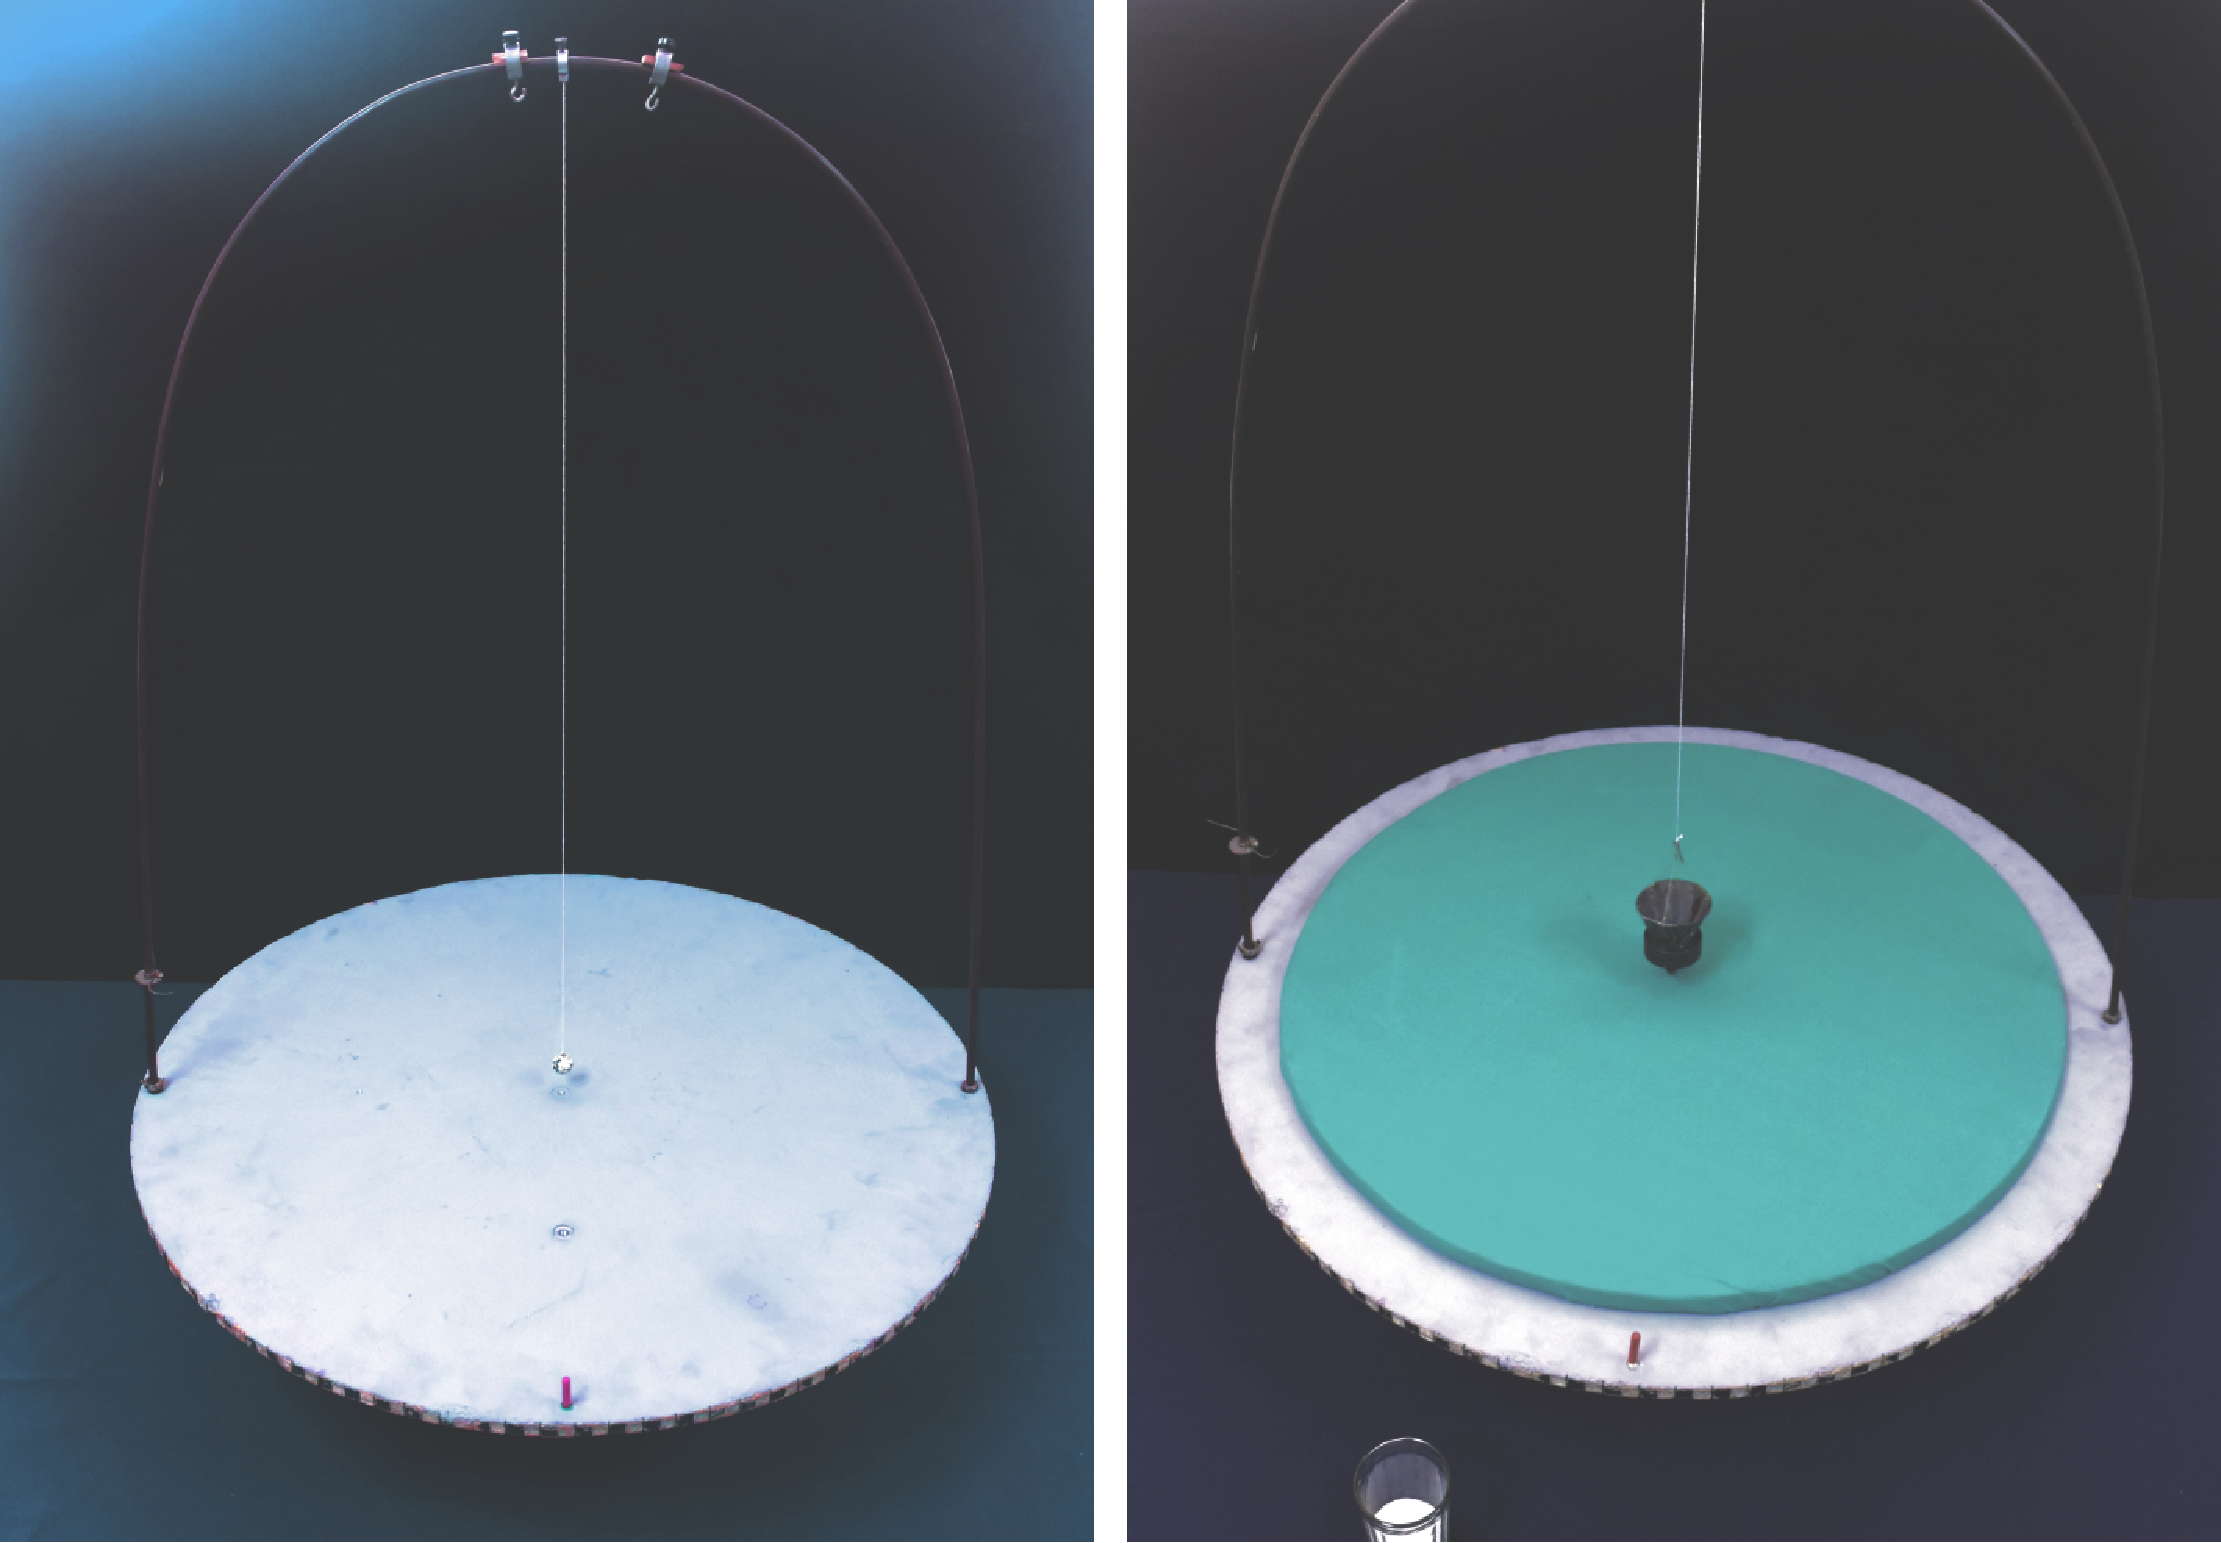
\includegraphics[width=0.9\linewidth]{fuko-1.png}
	\caption{Демонстрация способности математического маятника сохранять плоскость качания в пространстве при вращении платформы}
	\label{fuko-1}
\end{figure}
	
	\subsection*{\underline{Оборудование:}}

		\begin{enumerate}
			\item Платформа на вращающейся подставке
			\item Отвес на специальном штативе (шарик и воронка с песком)
			\item Маятник в виде ядра массой 20 кг, подвешенном за стальной трос к потолку
		\end{enumerate}

	\newpage
		\subsection*{\underline{Основные определения:}}
		
В середине XIX века Жан Бернард Леон Фуко смог провести опыт, который продемонстрировал суточное вращение Земли достаточно наглядно. 
Опыт этот был проведен неоднократно, а публично сам экспериментатор представил его в 1851 году в здании Пантеона в Париже.
									
Маятник Фуко - устройство, используемое для демонстраций, подтверждающих факт суточного вращения Земли.
Маятник представляет собой массивный груз, подвешенный на проволоке или нити, верхний конец которой укреплен (например, с помощью карданного шарнира) так, что позволяет маятнику качаться в любой вертикальной плоскости. 
Если маятник Фуко отклонить от вертикали и отпустить без начальной скорости, то, 
			поскольку действующие на груз маятника силы тяжести и натяжения нити лежат все время в плоскости качаний маятника и не могут вызвать ее вращения, эта плоскость будет сохранять неизменное положение
			по отношению к звездам (к инерциальной системе отсчета, связанной со звездами). 
			
В основу опыта был положен уже известный в то время экспериментальный факт: 
плоскость качания маятника на нити сохраняется независимо от вращения основания, к которому подвешен маятник. 
Маятник стремится сохранить параметры движения в инерциальной системе отсчета, плоскость которой неподвижна относительно звезд. 
На плоскость вращения маятника влияет как географическая широта места, где он установлен, так и длина подвеса (длинные маятники вращаются быстрее).	
Если поместить маятник Фуко на полюсе, то при вращении Земли плоскость маятника будет 
оставаться неизменной, и наблюдатели, вращающиеся вместе с планетой, должны видеть, 
как плоскость качаний маятника поворачивается без воздействия на него каких-либо сил. 
Таким образом, период вращения маятника на полюсе равен периоду обращения Земли вокруг своей оси – 24 часам. 
На других широтах период будет несколько больше, т. к. на маятник действуют силы инерции, возникающие во вращающихся системах – силы Кориолиса. 
На экваторе плоскость маятника вращаться не будет – период равен бесконечности.

	\newpage
	\subsection*{\underline{Краткое описание:}}
	
	Убедиться в способности маятника сохранять плоскость колебаний в пространстве можно при помощи специальной модели, состоящей 
	из небольшого маятника в виде шарика на нити 20—30 мм (рис.\ref{fuko-2}), подвешенного над круглой платформой, вращающимся на центробежной машине.
	Диаметр вращающейся платформы такой же, как в опыте с отвесами.
	
	\begin{figure}[H] 	
		\centering 	
		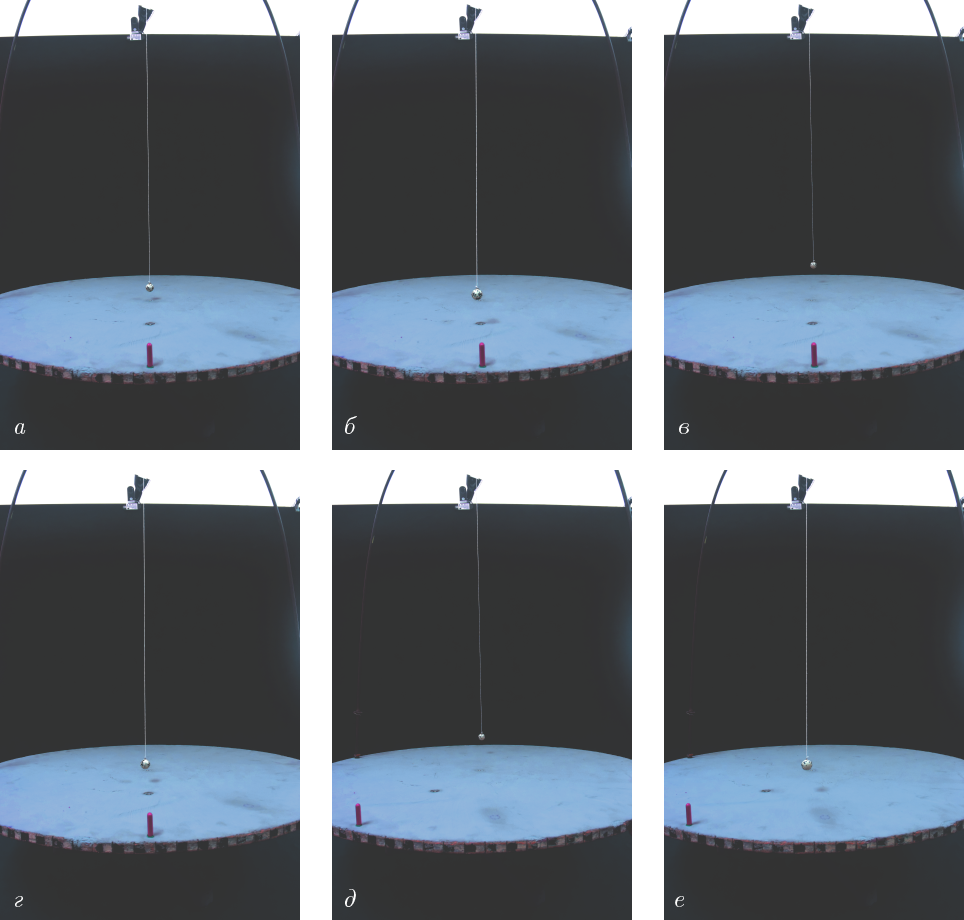
\includegraphics[width=0.6\linewidth]{fuko-2.png}
		\caption{Опыт с шариком демонстрирует сохранение плоскости качания маятника при вращении платформы}
		\label{fuko-2}
	\end{figure}
	
	Шарик крепится к специальной опоре в виде дуги из проволоки за нить длиной 70 см.
	После начала движения маятник в плоскости подвеса платформа приводится в равномерное вращение.
	При этом можно наблюдать, как плоскость колебания маятника по отношению к аудитории остается неизменной.
	Наблюдатель же, находящийся на Земле и вращающийся вместе с ней, 
	будет видеть, что плоскость качаний маятника медленно поворачивается относительно земной 
	поверхности в сторону, противоположную направлению вращения Земли.
	Этим и подтверждается факт суточного вращения Земли.
		
	Этот опыт можно показать с воронкой, из который на платформу высыпается песок.
	После полного оборота высыпавшийся песок изобразит на платформе несколько фигур, в зависимости от того, какой была скорость вращения платформы.
	Период качаний маятника в ходе опыта не изменяется.
	
\begin{figure}[H] 	
	\centering 	
	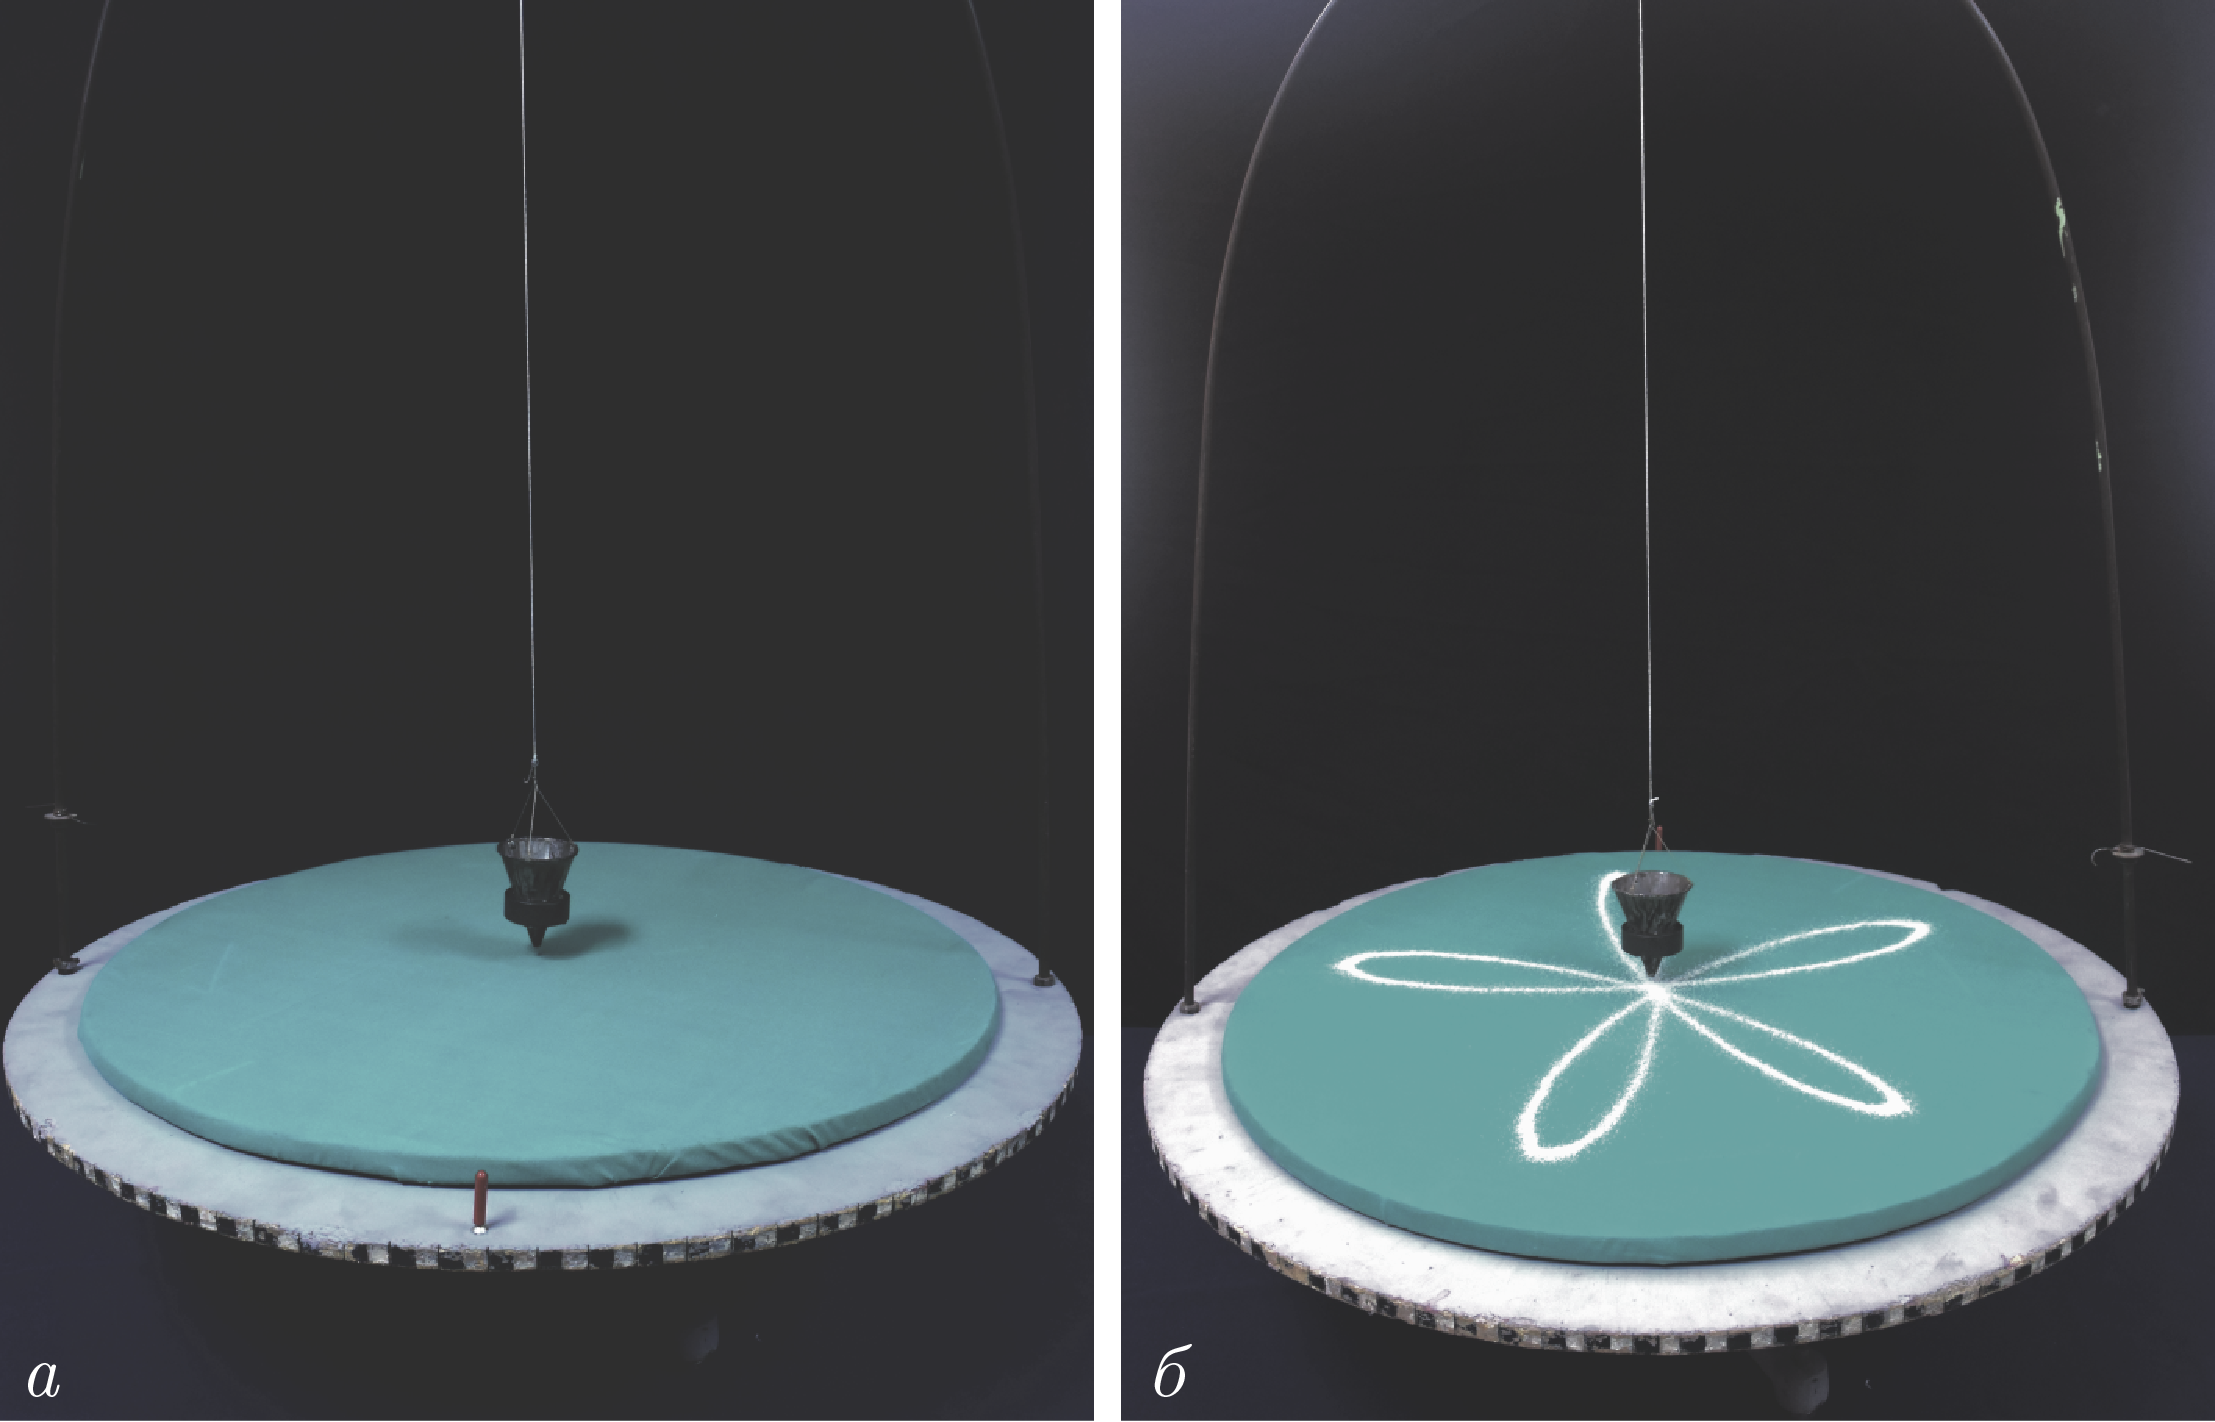
\includegraphics[width=0.8\linewidth]{fuko-3.png}
	\caption{Розетка, получаемая при записи качаний маятника во вращающейся системе. В представленном случае платформа начинала вращаться при прохождении маятником положения равновесия}
	\label{fuko-3}
\end{figure}

	
\newpage
	\subsection*{\underline{Теория:}}
	
	Представим себе маятник, помещенный над Северным полюсом Земли (рис.\ref{fuko-4}) на длинном, свободно вращающемся подвесе.
	Отведем его из положения равновесия и дадим возможность свободно качаться.
	Маятник движется под действием силы тяжести и натяжения подвеса.
	Обе они лежат в плоскости качания маятника, следовательно, плоскость качания должна сохранять свое положение в пространстве.
	Земля же поворачивается под маятником.
	проекция плоскости качания на поверхность Земли у полюса поворачивается в направлении, противоположном вращению Земли, со скоростью 15 градусов в час.
	Таким образом, в неподвижной системе отсчета поворот проекции плоскости качания маятника есть результат постоянства положения плоскости качания и вращения относительно Земли.
	
	\begin{figure}[H] 	
		\centering 	
		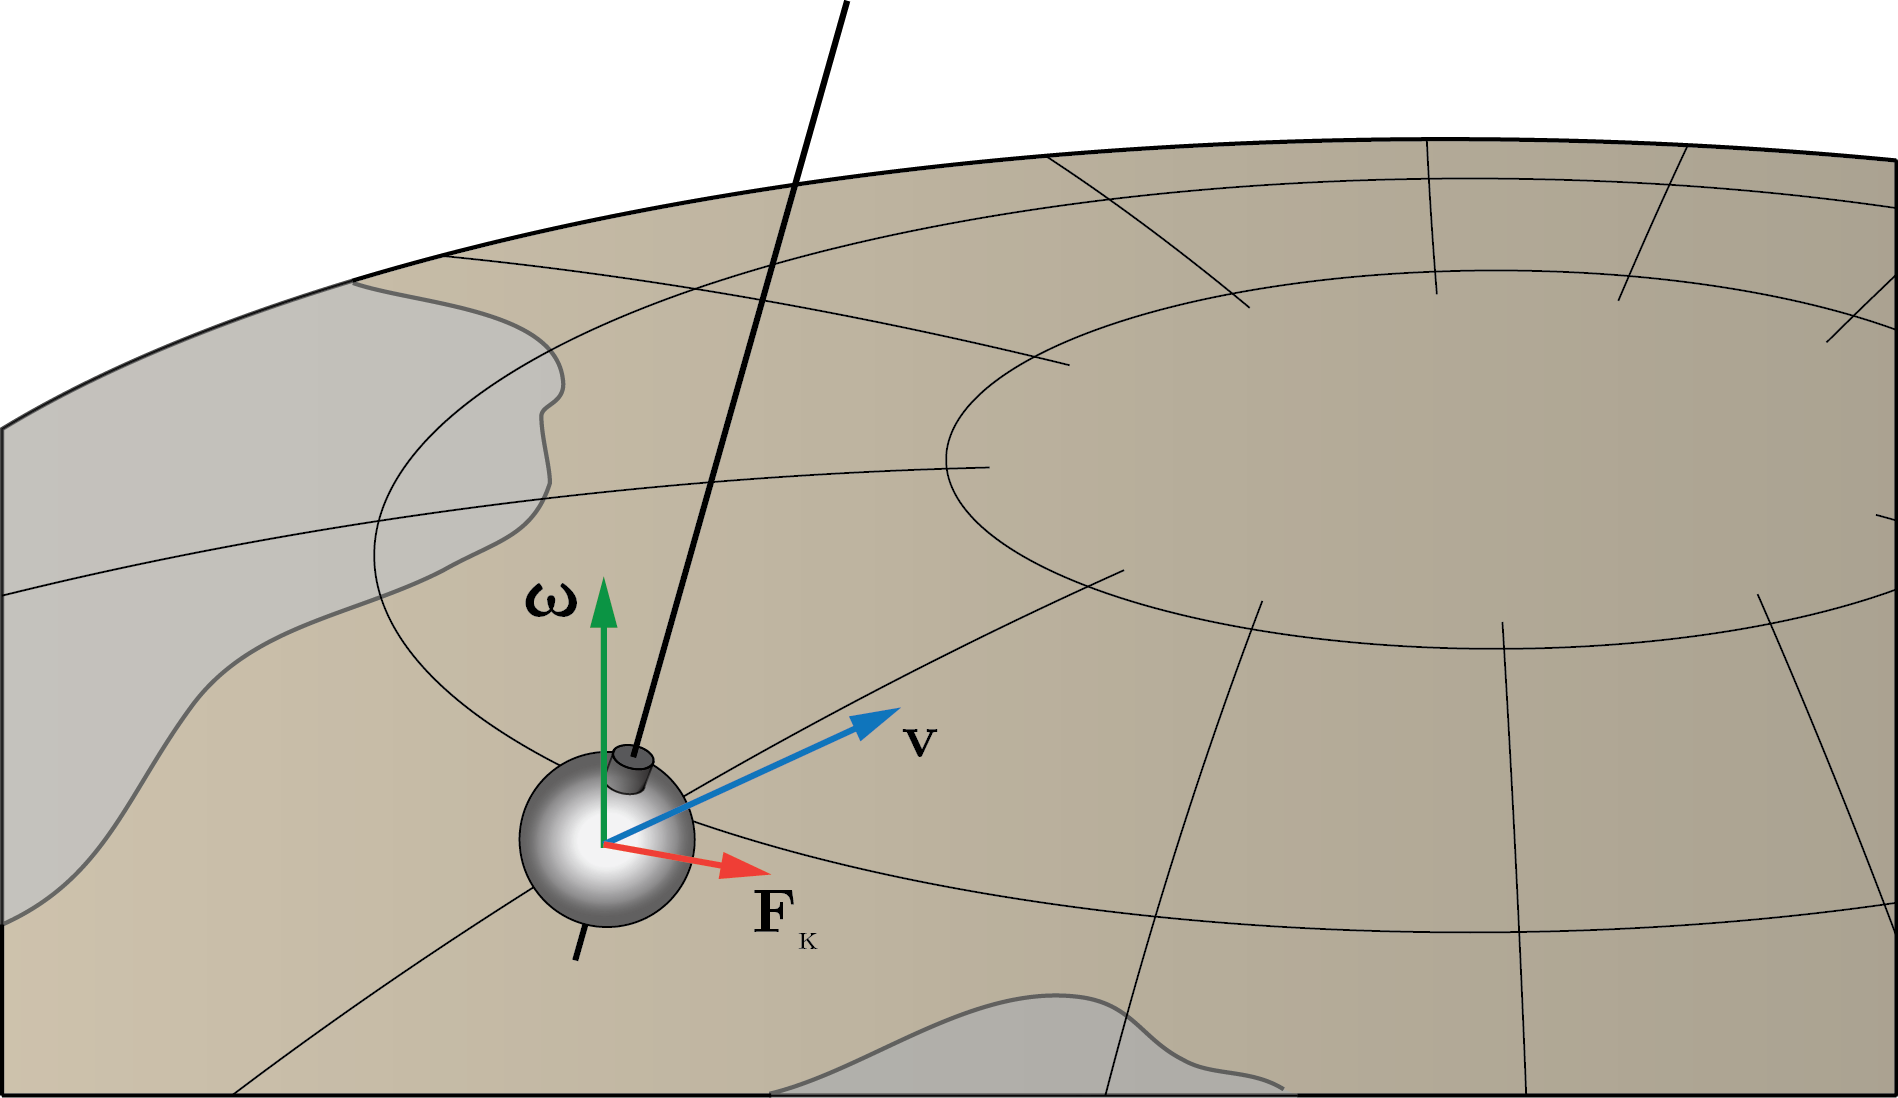
\includegraphics[width=0.75\linewidth]{fuko-4.png}
		\caption{Схема опыта Фуко}
		\label{fuko-4}
	\end{figure}
		
	Рассматривая движение маятника в системе координат, связанной с Землей, необходимо к указанным выше силам добавить силу Кориолиса.
	На полюсе скорость маятника \textbf{v} при большой длине подвеса можно считать перпендикулярной оси вращения Земли и, следовательно, вектору угловой скорости \textbf{ω}.
	Сила Кориолиса, действующая на маятник, будет равна 
	$ F_{\text{к}} = 2mv\omega $.
	
	Будучи перпендикулярной плоскости, включающей векторы $ v $  и $ \omega $, эта сила инерции лежит в горизонтальной плоскости и в соответствии с правилом буравчика направлена вправо от направления движения маятника. 
	Так как сила Кориолиса никакой другой силой не уравновешивается, она заставляет поворачиваться плоскость качания маятника по часовой стрелки (рис.\ref{fuko-5}).

	\begin{figure}[H] 	
		\centering 	
		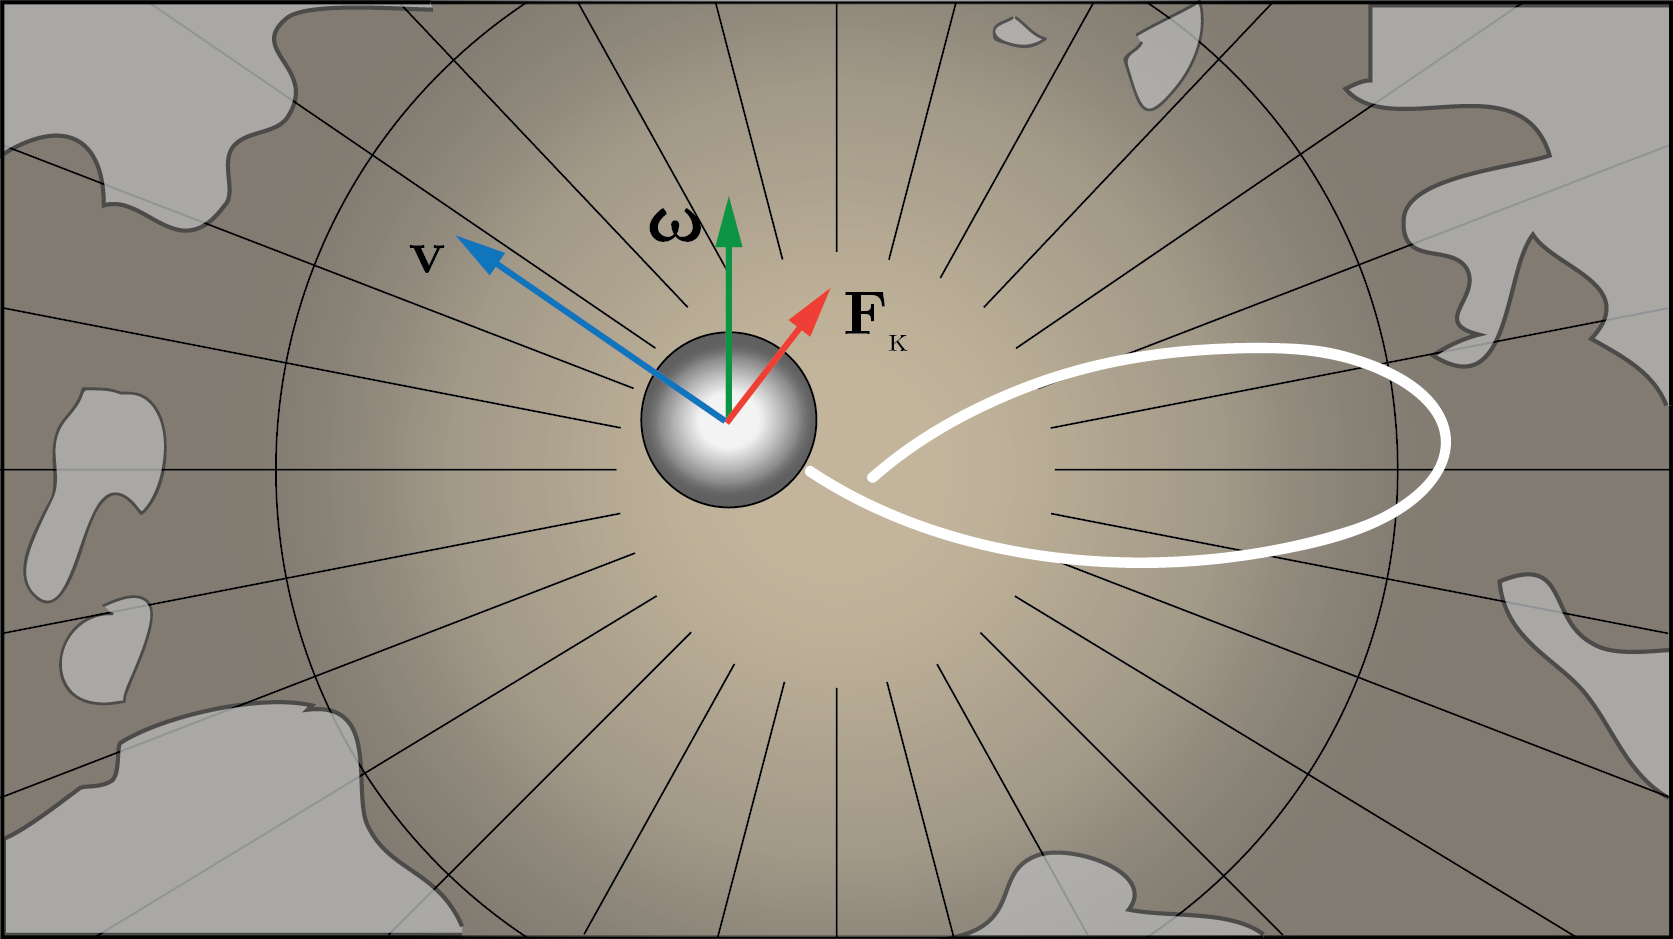
\includegraphics[width=0.75\linewidth]{fuko-5.png}
		\caption{Схематичное изображение траектории маятника, которую описывает на поверхности Земли груз, совершающий колебания на северном полюсе}
		\label{fuko-5}
	\end{figure}
	
	Можно сделать следующее замечание по поводу выбора размеров маятника для демонстрации опыта Фуко. 
	
	Если наибольшее отклонение $ l $ при качании маятника мало по сравнению с его длиной $ L $, то есть $ l \ll L $, то исходя из этого можно считать колебания гармоническими.
	Для таких колебаний период определяется следующим выражением:
	\begin{equation}\label{fuko-1eq1}
	T = 2\pi \sqrt{\frac{L}{g}}
	\end{equation}
	
	Запишем время затухания $ t $ в виде $ t = nT $
	\begin{equation}\label{fuko-1eq2}
	t = nT,
	\end{equation}
	где $ n $ — число колебаний маятника.
	
	Разумно положить, что по порядку величины $ n $ определяется отношением максимального значения потенциальной энергии маятника к среднему значению работы $ \bar{A} $ силы сопротивления за период колебаний:
	 \begin{equation}\label{fuko-1eq3}
	 n \sim \frac{U}{\bar{A}}
	 \end{equation}
	 
	В каждый момент сила сопротивления, действующая на груз со стороны воздуха, представляет собой:
	\begin{equation}\label{fuko-1eq4}
	F_{c} = \rho v^{2}R^{2},
	\end{equation}
	где $ \rho_{\text{в}} $ — плотность воздуха, $ v $ — мгновенная скорость, $ R $ — линейный размер груза.
	
	Выполняя операция осреднения, получим
	\begin{equation}\label{fuko-1eq5}
	\bar{v^{2}} = \frac{1}{2}\omega^{2}l^{2},
	\end{equation}
	где $ \omega = \sqrt{g/L} $ — циклическая частота колебаний.
	Тогда $ \bar{F_{c}}  = \rho_{\text{в}} R^{2}\omega^{2}l^{2} $ и $ \bar{A} = \rho_{\text{в}} R^{2}\omega^{2}l^{2} $.
	
	Далее можно показать, что максимальная высота подъема маятника
	\begin{equation}\label{fuko-1eq6}
	H = L - L \cos\alpha \approx \frac{l^{2}}{2L},
	\end{equation}
	и
	\begin{equation}\label{fuko-1eq7}
	U \approx\frac{ Mgl^2}{2L} \sim \frac{\rho g R^{3}l^{2}}{2L},
	\end{equation}
	где $ M $ - масса груза, $ \rho $ — его плотность. 
	
	В результате получаем искомое время затухания маятника Фуко:
	\begin{equation}\label{fuko-1eq8}
	t = nT \sim  \frac{U}{\bar{A}}T \sim\sqrt{\frac{L}{g}} \frac{\rho}{\rho_{\text{в}}}\frac{R}{l}
	\end{equation}
	
	Именно в этом выражении заключается ответ на замечание по поводу параметров подвеса для демонстрации опыта Фуко.
	Рассмотрев маятник, линейные размеры которого меньше используемого в данной демонстрации в 100 раз.
	Согласно выражению (\ref{fuko-1eq8}) время затухания $ t $ для такого маятника уменьшится в 10 раз, а, соответственно, ослабнет эффект вращения плоскости колебаний.
	По этой причине для демонстрации суточного вращения Земли применяется маятник Фуко в виде массивного ядра на очень большом подвесе.
	
\end{document}
